\chapter{Work Done}

\section{With FOSSCell}
FOSSCell (Free and Open Source Software Cell)\textsuperscript{\cite{fosscell}} of NIT Calicut is a group of enthusiasts in the NITC campus who believe in the ideology of free and open source software. FOSSCell organizes events for promotion of FOSS, workshops and talks that allow masses to learn alternative software like GNU/Linux, Python, etc.

\subsection{Orientation Program 2010}
An orientation program for the freshers of the institute was done on September 7, 2010\textsuperscript{\cite{orientation}}. Information about what is Free and Open Source Software, Google Summer of Code and FOSSCell of NIT Calicut was given along with screening of some informative videos related to FOSS. Many freshers attended the orientation.

\subsection{Exhibition at the National Conference on Free Software in Education}
National Conference on Free Software and Education\textsuperscript{\cite{fsinedu}} was organized during September 10-12, 2010 by Free Software Foundation of India\textsuperscript{\cite{fsfi}}; SPACE, Thiruvananthapuram\textsuperscript{\cite{space}}; and National Institute of Technology Calicut. Richard Stallman, the founder of GNU project and the Free Software Foundation, inaugurated the conference. During the first day of the conference, one of us co-ordinated an exhibition done by freshers in which stalls were setup to spread awareness about free software like Blender, Inkscape, Ubuntu, GIMP, etc. In the exhibition, a demo of localization under GNU/Linux environment in various Indian languages was also done alongwith a presentation on FOSS. Some photos are available online\textsuperscript{\cite{fsinedupics}}.

\subsection{Celebration of Software Freedom Day}
Software Freedom Day is a worldwide celebration of Free and Open Source Software. The goal in this celebration is to educate the worldwide public about the benefits of using high quality FOSS in education, in government, at home, and in business.

SFD was celebrated at the NITC campus on September 18, 2010\textsuperscript{\cite{sfd}}. During the program information about Software Freedom was given to participants and some hand outs containing information about various free software were also distributed. Before and after the celebration, various posters related to free and open source software were pasted in places like Mini Canteen and hostels including the Ladies Hostel.

\subsection{Setting up of FOSSHut @ Tathva 2010}
A FOSSHut was setup in one of the exhibition halls during Tathva 2010\textsuperscript{\cite{tathva}} during October 22 to 24, 2010. It featured a Freedom Toaster (which allows anyone to burn disks of any GNU/Linux distro for free) brought by Zyxware Technologies\textsuperscript{\cite{zyxware}}, some promotional material by SPACE, various GNU/Linux Desktop Demos, Free and Open Source Software Demos, information about Creative Commons and quality free and open source software through posters and interaction, a GNU/Linux Install Fest, Screening of Open Movies, Games on Linux, and an Unconference. It was volunteered by many freshers and other members of FOSSCell. Some photographs are available online\textsuperscript{\cite{fosshutpics}}.

\subsection{A Demo session on Drupal}
A demo session on Drupal - an open source content management platform, was conducted by one of us to help interested people (including freshers and FOSSCell members) learn about basics of Drupal on November 6, 2010\textsuperscript{\cite{drupaldemo}}.

\section{A Survey on Software Ethics Awareness}
We created a survey on Software Ethics Awareness to spread awareness about ethics related to software and also to analyze the current situation in NIT Calicut. Survey was conducted both online and offline.

The online survey was done with the help of a website \url{http://www.surveymonkey.com/}. Online participants included NITC students who are users of social networking websites like Facebook and Twitter, students of our batch and also some of the FOSSCell members. They belonged to various courses, branches and years of study. The survey was done during October 27 to November 4, 2010 (about 8 days) and we received responses of 77 participants.

For offline survey we distributed 200 paper copies among the freshers and some other group of students (the paper version of the survey can be seen at the end of this document). This at least had the effect of spreading awareness among the respondents. We realized on collection of the survey forms that manual analysis of the offline survey data was a next to impossible task. So, here we present the observations from the online survey only:

\begin{figure}[h!]
\centering
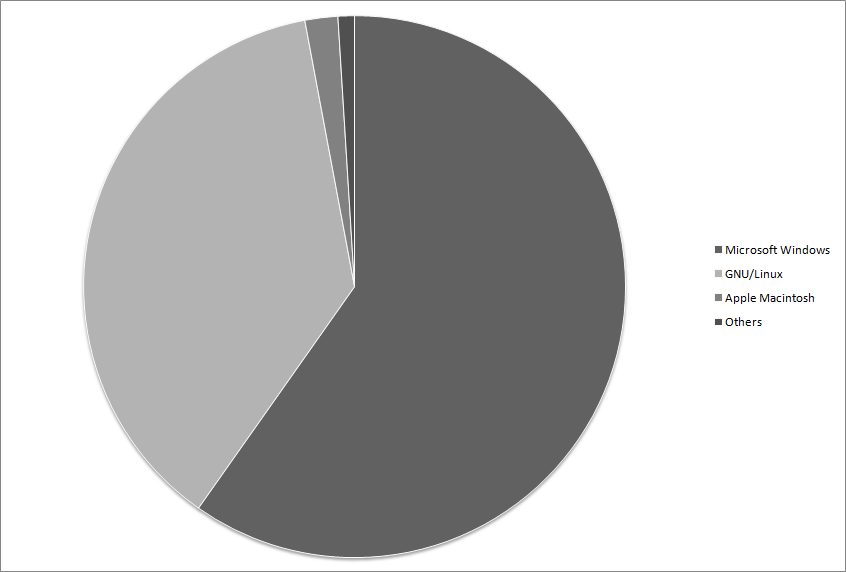
\includegraphics[width=0.8\textwidth]{./q1.png}
\caption{Operating System usage}
\label{fig:q1}
\end{figure}

\emph{Figure~\ref{fig:q1}:} What operating one is using usually says much about the tendency to use illegal copies of software. It has been observed, generally, that most of the illegal sharing of software happens on the Windows platform. Here we observed that a good share of students are using other operating systems also.

\newpage
\begin{figure}[h!]
\centering
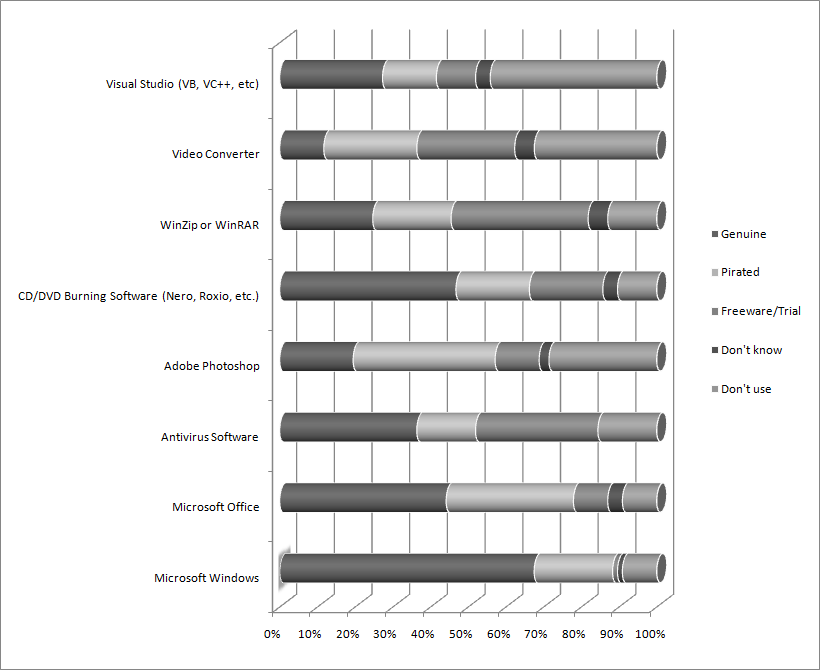
\includegraphics[width=0.8\textwidth]{./q2.png}
\caption{Classification of common software used}
\label{fig:q2}
\end{figure}

\emph{Figure~\ref{fig:q2}:} In the second question that we asked we tried to analyze usage patterns for common software. It can be observed that Microsoft Windows and CD/DVD Burning Software such as Nero or Roxio are the two software that are being used as legal copy. The reason for this can be attributed to bundling of licensed versions of these software with most of the laptops available these days. The most used pirated software are Microsoft Office and Adobe Photoshop. Compression software and Antivirus software are the two most used in freeware or trial category.

\newpage
\begin{figure}[h!]
\centering
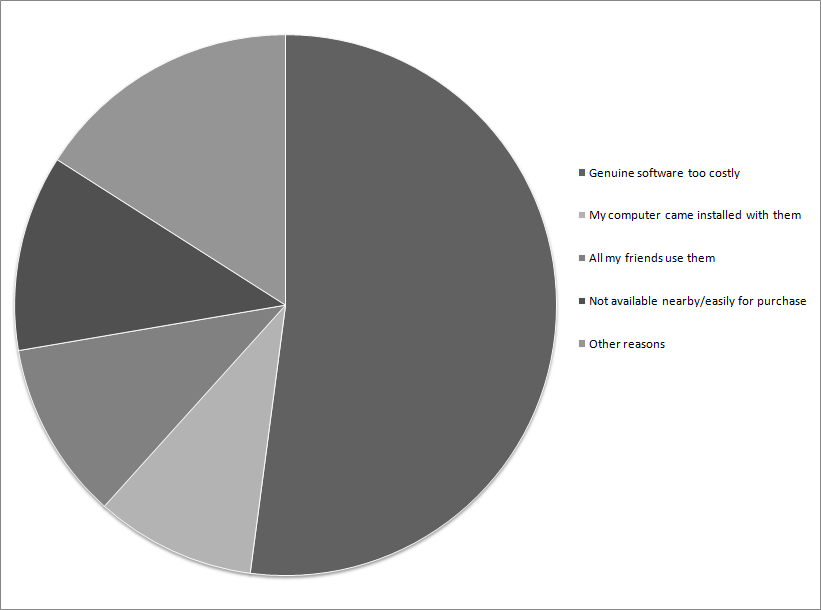
\includegraphics[width=0.8\textwidth]{./q3.png}
\caption{Reasons for using pirated software}
\label{fig:q3}
\end{figure}

\emph{Figure~\ref{fig:q3}:} Here we tried to find out why people tend to use illegal copies of software. More than half of those responded believe that genuine software is too costly. Almost equivalent proportion of people attributed it to the next 3 reasons. Other prominent reasons included: they don't use pirated software, need for some project work, and pirated software easily/freely available.

\newpage
\begin{figure}[h!]
\centering
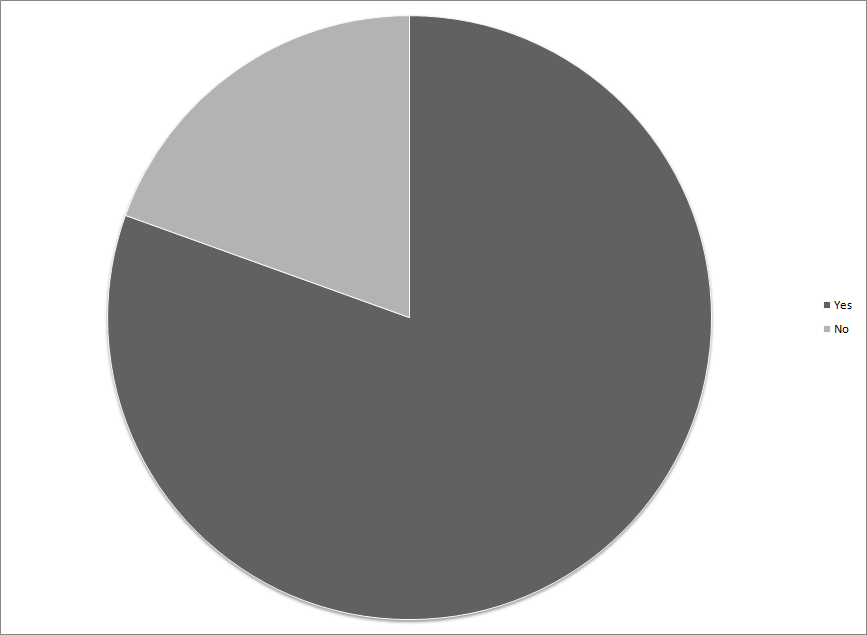
\includegraphics[width=0.8\textwidth]{./q4.png}
\caption{Awareness of consequences}
\label{fig:q4}
\end{figure}

\emph{Figure~\ref{fig:q4}:} Over three-fourths of the proportion were aware that using, copying or distributing illegal copies of software can land them up in jail.

\newpage
\begin{figure}[h!]
\centering
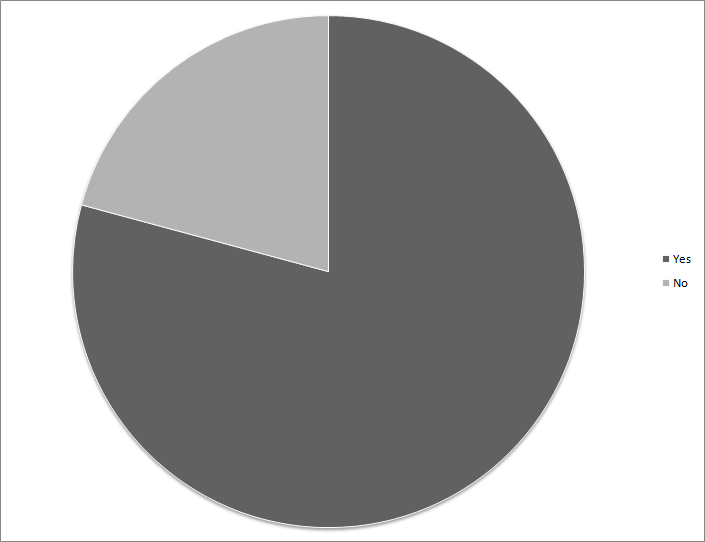
\includegraphics[width=0.8\textwidth]{./q5.png}
\caption{Awareness of existence of alternatives}
\label{fig:q5}
\end{figure}

\emph{Figure~\ref{fig:q5}:} Almost same percentage of respondents as in the previos question were aware about the existence of free and open source software alternatives.

\newpage
\begin{figure}[h!]
\centering
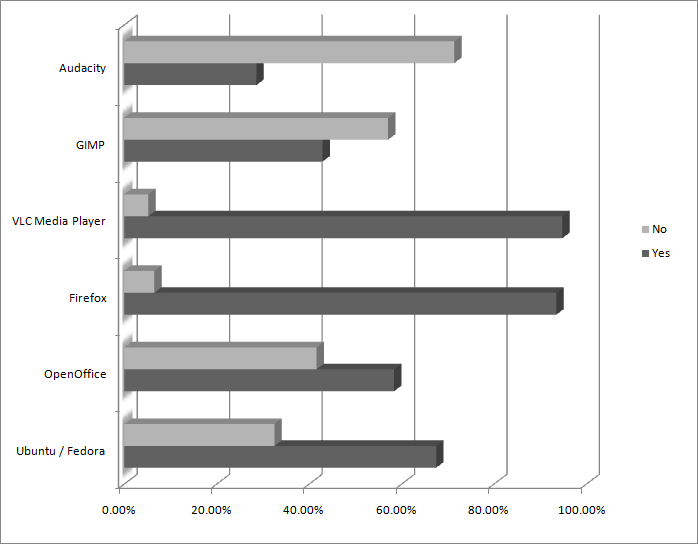
\includegraphics[width=0.8\textwidth]{./q6.png}
\caption{Common FOSS usage}
\label{fig:q6}
\end{figure}

\emph{Figure~\ref{fig:q6}:} VLC Media Player and Firefox come out as the most popular free or open source software being used, followed by Ubuntu/Fedora and OpenOffice.
\newpage
\begin{figure}[h!]
\centering
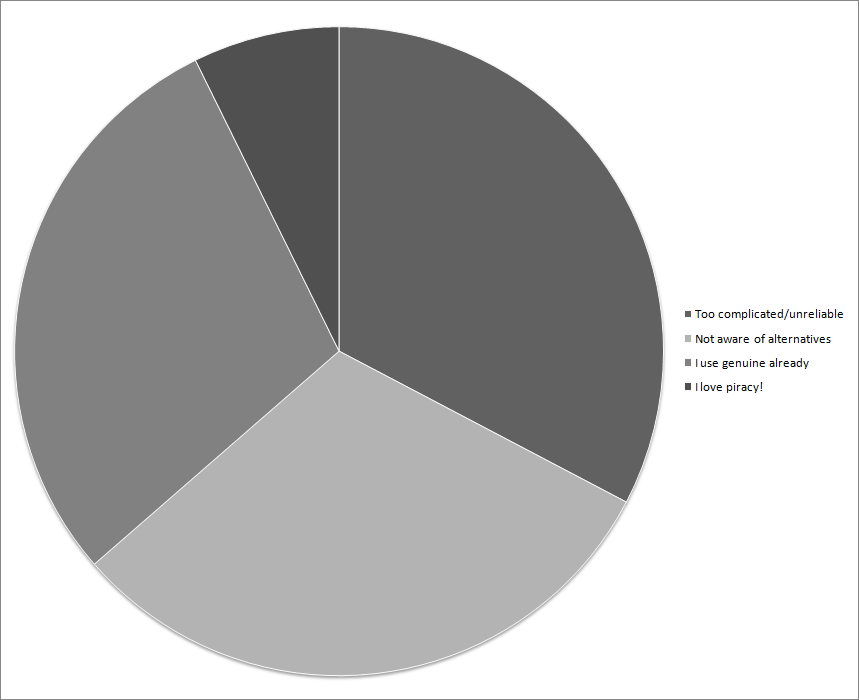
\includegraphics[width=0.8\textwidth]{./q7.png}
\caption{Reasons for not using FOSS}
\label{fig:q7}
\end{figure}

\emph{Figure~\ref{fig:q7}:} Almost equal percentages of people cited the first three options as the reason for not using free and open source software alternatives. Alas, there is also a small percentage of people who love piracy!
\newpage
\begin{figure}[h!]
\centering
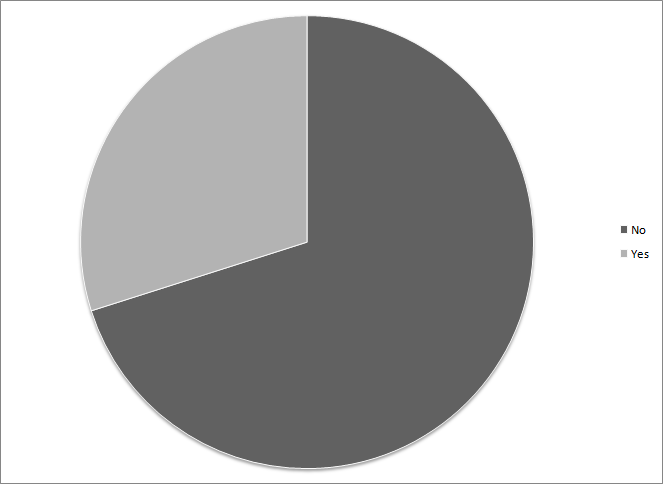
\includegraphics[width=0.8\textwidth]{./q8.png}
\caption{Support for piracy}
\label{fig:q8}
\end{figure}

\emph{Figure~\ref{fig:q8}:} Over 70\% of respondents responded in negative when asked ``Do you support piracy?''.\ They were asked to write some reason if they chose `No', some of the reasons mentioned were: cost issues, educational reasons, no alternatives, ease of use. One respondent even mentioned that until she starts earning to buy genuine, she will use pirated software.
\newpage
\begin{figure}[h!]
\centering
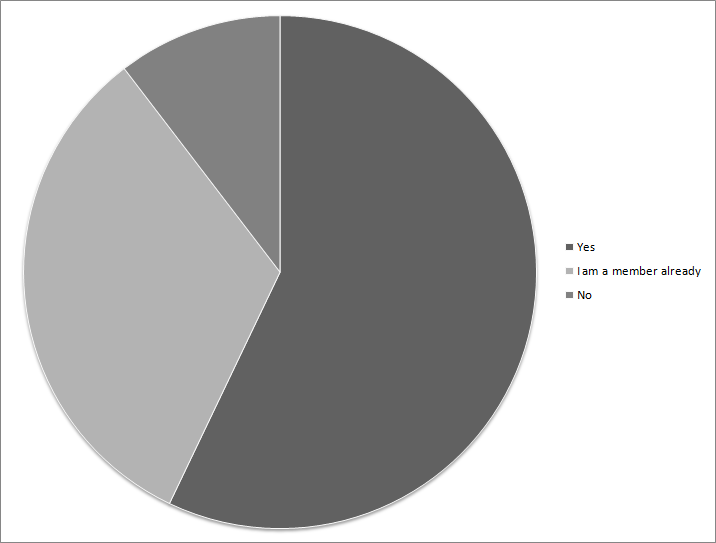
\includegraphics[width=0.8\textwidth]{./q9.png}
\caption{Awareness about FOSSCell}
\label{fig:q9}
\end{figure}

\emph{Figure~\ref{fig:q9}:} This question was selected to find out if students knew about a support group that is active in the campus itself. This also establishes that almost one-third of the survey respondents were FOSSCell members. Other than them, almost 60\% of respondents were aware of the existence of FOSSCell.
